% !TeX program = xelatex
% Bản thảo độc lập để duyệt; chưa được ghép vào báo cáo tổng.
\documentclass[conference]{IEEEtran}

\usepackage{fontspec}
\usepackage[english,vietnamese]{babel}
\defaultfontfeatures{Ligatures=TeX}
\usepackage{amsmath,amssymb}
\usepackage{booktabs}
\usepackage{graphicx}
\usepackage[hidelinks]{hyperref}
\graphicspath{{figures/tv3_k32_bovw/}}

\title{Cơ sở lựa chọn cấu hình $K=32$ và BoVW nhị phân cho khai phá mẫu trên Fashion-MNIST}
\author{\IEEEauthorblockN{Thành viên 3}}

\begin{document}
\selectlanguage{vietnamese}
\maketitle

\section{Lựa chọn cấu hình phân cụm và biểu diễn giao dịch}
\label{sec:tv3_k32_selection}

\subsection{Tiêu chí lựa chọn}

Thí nghiệm khảo sát năm kích thước từ điển $K\in\{16,32,64,128,256\}$, mỗi kích thước được chạy với ba seed. Do mục tiêu của phần này là khai phá và diễn giải các tập mục thường xuất hiện, cấu hình được chọn cần cân bằng giữa độ chi tiết của từ điển và độ gọn của giao dịch, đồng thời giữ cho số mẫu cần xem xét ở mức có thể quản lý. Độ méo thấp hơn hoặc số tập mục nhiều hơn, nếu đứng riêng lẻ, chưa đủ để kết luận cấu hình đó có ý nghĩa thị giác hay giá trị dự đoán tốt hơn.

\subsection{So sánh kích thước từ điển}

Cả 15 lượt fit đều hội tụ và sử dụng đủ số cụm đã đặt. Độ méo trung bình giảm từ $0{,}4463$ tại $K=16$ xuống $0{,}3488$ tại $K=32$ và $0{,}2720$ tại $K=64$. Xu hướng này phù hợp với việc tăng số tâm giúp mô tả dữ liệu huấn luyện chi tiết hơn. Tuy nhiên, mức giảm tương đối giữa $K=16$ và $K=32$ là khoảng $21{,}8\%$, gần với mức $22{,}0\%$ giữa $K=32$ và $K=64$; do đó, số liệu không cho thấy một điểm gãy rõ ràng tại $K=32$.

Quyết định chọn $K=32$ dựa trên độ gọn của biểu diễn và khối lượng mẫu cần rà soát. Với BoVW nhị phân, độ dài giao dịch trung bình tăng từ $8{,}82$ mục ở $K=16$ lên $12{,}26$ mục ở $K=32$, rồi lên $15{,}04$ mục ở $K=64$. Ở cùng ngưỡng hỗ trợ 3\% và giới hạn độ dài hai, số tập mục gồm hai mã trung bình lần lượt là $120$, $487{,}3$ và $1.451{,}3$. Như vậy, $K=32$ tạo được khoảng bốn lần số cặp của $K=16$, trong khi vẫn tạo ít hơn khoảng hai phần ba số cặp so với $K=64$. Mức tăng ở $K=64$ đi kèm độ méo thấp hơn, nhưng cũng làm giao dịch dài hơn khoảng $22{,}6\%$ và số cặp cần xem xét tăng gần ba lần so với $K=32$.

Các giá trị lớn hơn không làm số cặp tăng đều: $K=128$ tạo trung bình $1.489{,}7$ cặp, còn $K=256$ tạo $638{,}3$ cặp dù giao dịch dài nhất trong các cấu hình được khảo sát. Đây là dấu hiệu cho thấy việc tăng kích thước từ điển có thể phân tán các mã và làm thay đổi độ phổ biến của tổ hợp; riêng số đếm này không chứng minh chất lượng ngữ nghĩa của từ điển.

\begin{table}[!t]
    \centering
    \caption{Độ méo và đặc trưng giao dịch BoVW nhị phân theo kích thước từ điển}
    \label{tab:tv3_k32_bovw_by_k}
    \scriptsize
    \setlength{\tabcolsep}{2.5pt}
    \begin{tabular}{@{}c c c r@{}}
        \toprule
        $K$ & $\bar{D}\pm s_D$ & $\overline{|T|}$ & $\bar{n}_2$ \\
        \midrule
        16  & $0{,}4463\pm0{,}0065$ & $8{,}82$  & $120{,}0$ \\
        32  & $0{,}3488\pm0{,}0037$ & $12{,}26$ & $487{,}3$ \\
        64  & $0{,}2720\pm0{,}0006$ & $15{,}04$ & $1.451{,}3$ \\
        128 & $0{,}2179\pm0{,}0005$ & $17{,}92$ & $1.489{,}7$ \\
        256 & $0{,}1769\pm0{,}0001$ & $20{,}37$ & $638{,}3$ \\
        \bottomrule
    \end{tabular}

    \vspace{2pt}
    \parbox{0.96\columnwidth}{\scriptsize Mỗi hàng lấy trung bình ba seed. $\bar{D}\pm s_D$: độ méo trung bình và độ lệch chuẩn; $\overline{|T|}$: độ dài giao dịch trung bình; $\bar{n}_2$: số cặp phổ biến trung bình tại minsup 3\% (2.100/70.000), giới hạn độ dài hai. Số cặp mô tả lượng kết quả cần rà soát, không đo trực tiếp chất lượng ngữ nghĩa.}
\end{table}

\begin{figure}[!t]
    \centering
    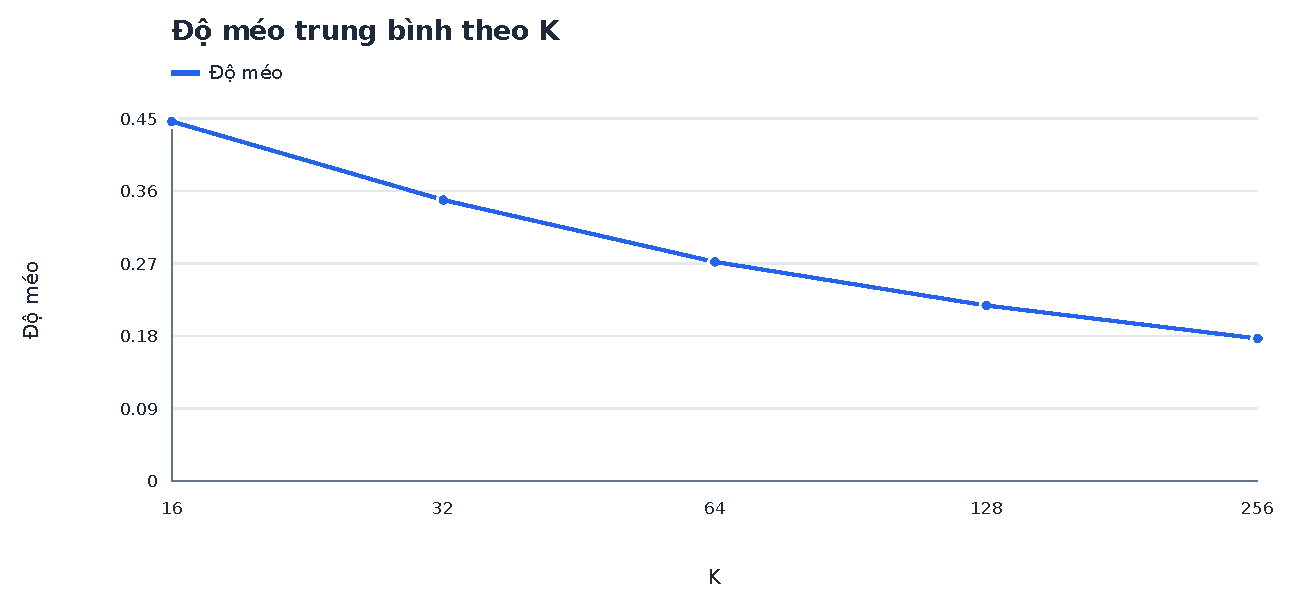
\includegraphics[width=\columnwidth]{kmeans_distortion.pdf}\\[2pt]
    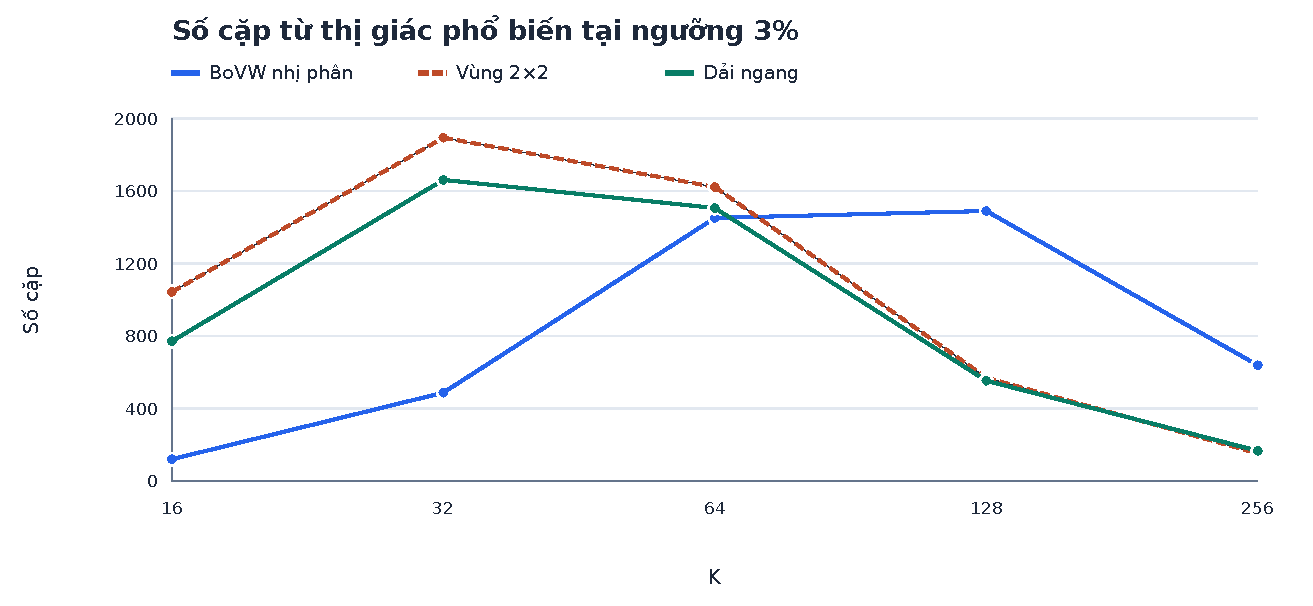
\includegraphics[width=\columnwidth]{frequent_pairs.pdf}
    \caption{Đối chiếu độ méo trung bình theo $K$ (trái) và số tập mục gồm hai mã tại ngưỡng hỗ trợ 3\% (phải). Đường BoVW nhị phân cho thấy số cặp thay đổi thế nào khi tăng kích thước từ điển; biểu diễn theo vùng 2$\times$2 và theo ba dải ngang được đưa vào để đối chiếu ảnh hưởng của vị trí.}
    \label{fig:tv3_k32_bovw_tradeoff}
\end{figure}

\subsection{Ý nghĩa của các cách biểu diễn giao dịch}

Mỗi ảnh được chia thành lưới $7\times7$ gồm 49 vị trí patch $4\times4$. Sau bước lọc nền, mỗi patch được giữ lại có một mã từ thị giác $w$ do codebook chung gán. BoVW nhị phân bỏ qua vị trí và chỉ giữ tập các mã khác nhau xuất hiện trong ảnh. Ba biến thể không gian dưới đây dùng cùng patch và mã từ thị giác đó, nhưng thay đổi thông tin được đưa vào từng mục giao dịch. Nhãn lớp được lưu riêng trong metadata, không tham gia tạo mục.

\textbf{Biểu diễn theo vùng 2$\times$2.} Lưới được cắt sau hàng 3 và cột 3 thành bốn vùng tuyệt đối: trên trái, trên phải, dưới trái và dưới phải. Mục có dạng $(R_i,w)$, tức mã từ thị giác $w$ xuất hiện trong vùng $R_i$. Vì lưới 7$\times$7 không chia đều, bốn vùng có lần lượt 9, 12, 12 và 16 vị trí patch. Cùng một mã từ xuất hiện ở hai vùng sẽ tạo hai mục khác nhau.

\textbf{Biểu diễn theo ba dải ngang.} Các hàng 1–2 tạo dải trên, hàng 3–5 tạo dải giữa, và hàng 6–7 tạo dải dưới. Mục có dạng $(B_j,w)$, trong đó $B_j$ là một trong ba dải. Số vị trí patch tương ứng là 14, 21 và 14; cùng một mã từ ở hai dải khác nhau cũng được xem là hai mục.

\textbf{Biểu diễn quan hệ lân cận cục bộ.} Thay vì gắn một mã từ với một vùng, cách này xét cặp patch phân biệt đã được giữ lại nếu khoảng cách Manhattan $d_{\mathrm{M}}=|r_a-r_b|+|c_a-c_b|$ thuộc $\{1,2\}$, với $(r_a,c_a)$ và $(r_b,c_b)$ là tọa độ của hai patch. Nếu hai patch khác hàng, hệ thống tạo mục \texttt{ABOVE} theo thứ tự từ patch phía trên đến patch phía dưới; nếu khác cột, tạo mục \texttt{LEFT\_OF} theo thứ tự từ trái sang phải. Vì vậy, một cặp chéo có thể sinh cả hai quan hệ. Hai patch khác nhau có thể mang cùng mã từ. Chỉ các cặp nằm trong lưới thật được xét: không nối hàng 7 với hàng 1 hoặc cột 7 với cột 1; patch bị lọc không tham gia tạo quan hệ.

Hình~\ref{fig:tv3_spatial_encodings} minh họa ba quy tắc trên cùng một lưới patch. Các mã $w_i$ trong hình chỉ là ví dụ để giải thích cách tạo mục, không phải nhãn lớp hoặc nhận diện ngữ nghĩa của một loại trang phục.

\begin{figure}[!t]
    \centering
    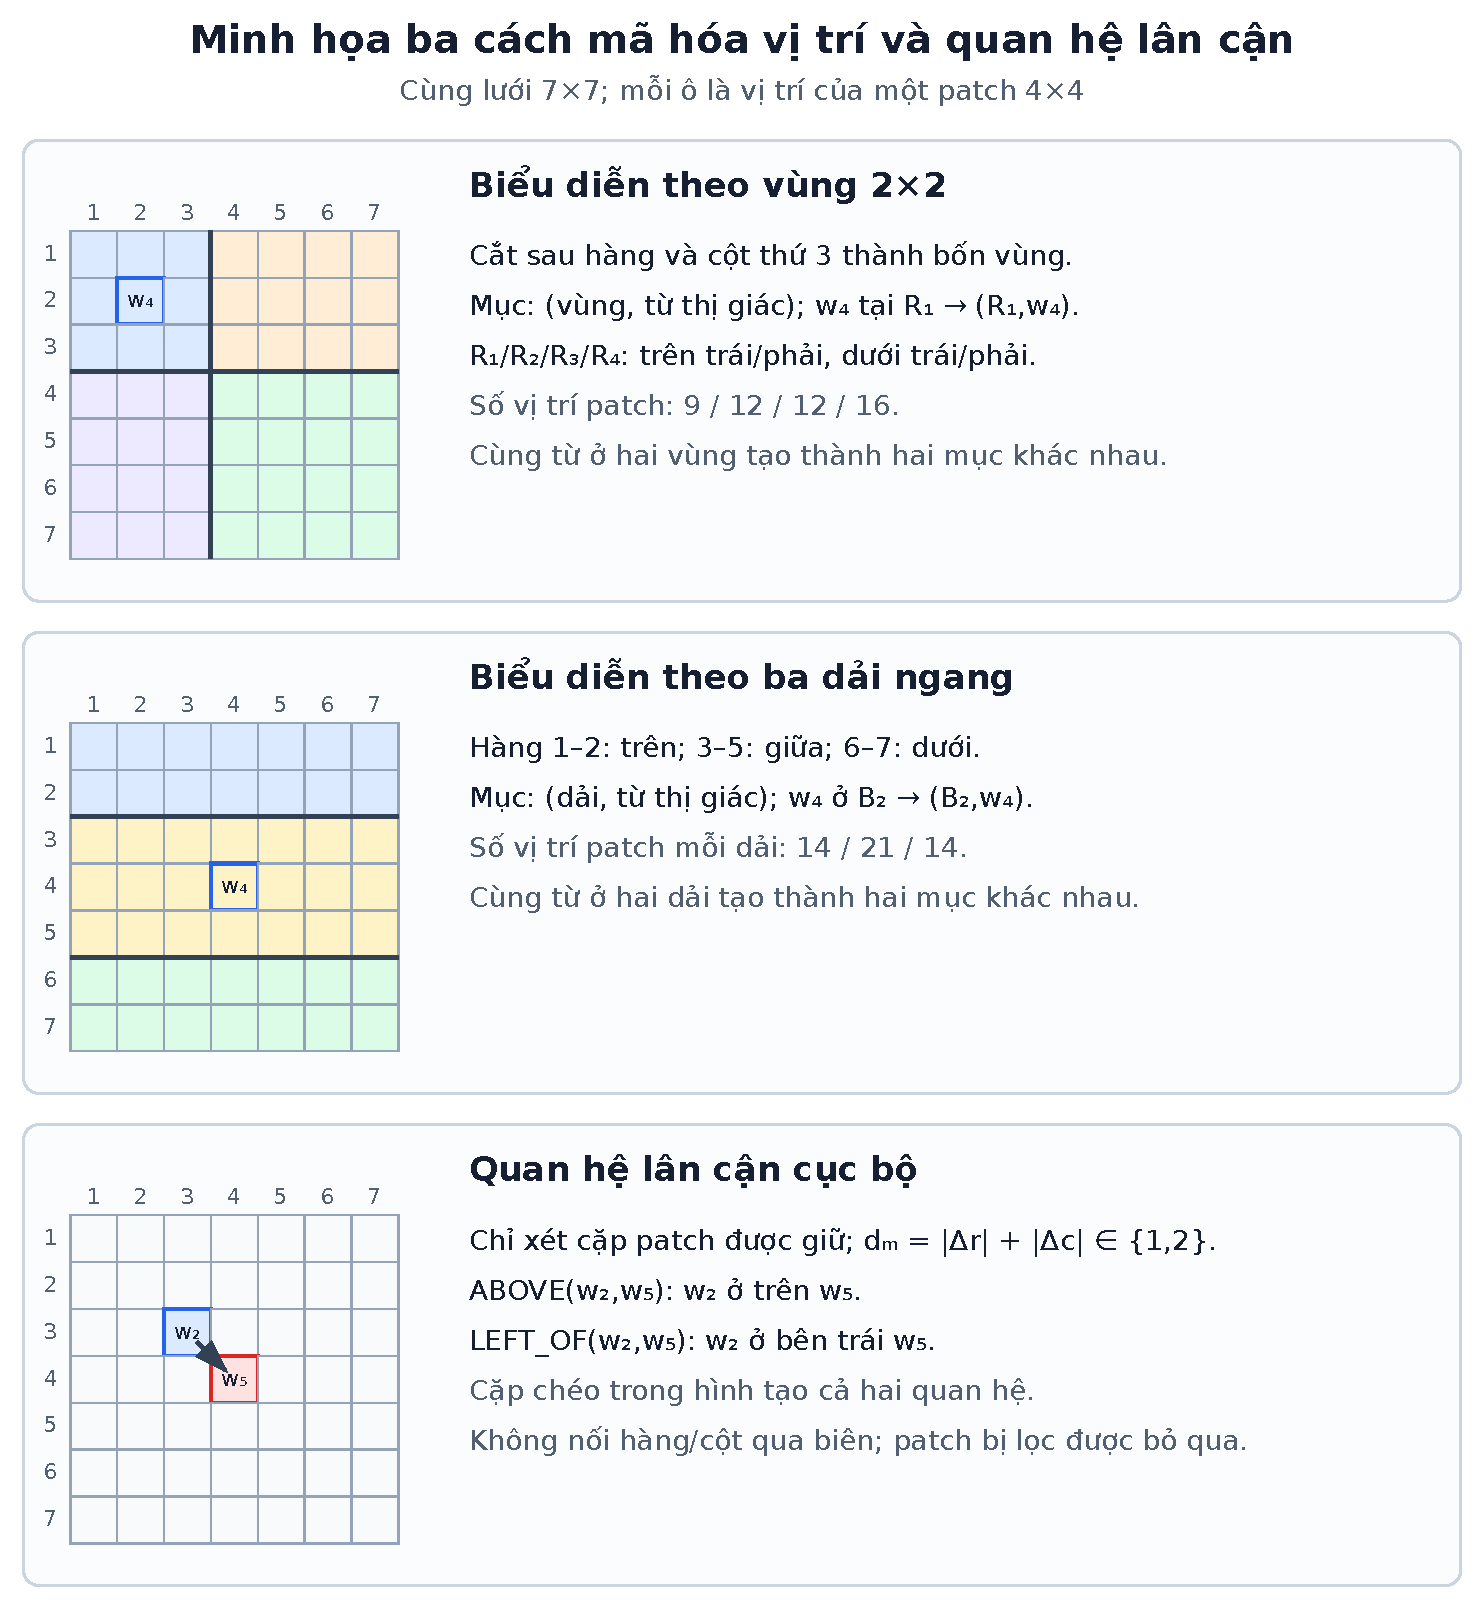
\includegraphics[width=\columnwidth]{spatial_encoding_schematic.pdf}
    \caption{Minh họa cách biểu diễn theo vùng 2$\times$2 gắn từ thị giác với vùng, biểu diễn theo ba dải ngang gắn từ với dải, và biểu diễn quan hệ lân cận cục bộ tạo quan hệ có hướng giữa các patch gần nhau. Mỗi ô là một vị trí patch; trong dữ liệu thực, chỉ patch vượt qua bước lọc mới có mã từ và tham gia tạo mục. Cặp chéo trong ví dụ cuối có khoảng cách Manhattan 2 nên tạo cả quan hệ phía trên và bên trái.}
    \label{fig:tv3_spatial_encodings}
\end{figure}

\subsection{Lựa chọn BoVW nhị phân}

BoVW nhị phân biểu diễn mỗi ảnh bằng tập các từ thị giác xuất hiện trong ảnh, mỗi từ chỉ được ghi một lần. Cách mã hóa này không giữ tọa độ vùng ảnh, nên câu hỏi khai phá được giới hạn rõ: những từ thị giác nào thường cùng có mặt trong một ảnh? Quy tắc này tạo một mốc cơ sở đơn giản để diễn giải và đối chiếu với các biến thể có xét vị trí.

Tại $K=32$, BoVW nhị phân có độ dài giao dịch trung bình $12{,}26$ mục. Với cùng ngưỡng và giới hạn khai thác, biểu diễn này tạo trung bình $487{,}3$ cặp; biểu diễn theo vùng 2$\times$2 và biểu diễn theo ba dải ngang lần lượt tạo $1.894$ và $1.661{,}3$ cặp. Số cặp lớn hơn ở hai biểu diễn có xét vị trí phản ánh việc chúng mở rộng tập mục và tạo thêm tổ hợp để xem xét; chỉ riêng số lượng đó không cho biết các tổ hợp có dễ diễn giải hơn hoặc có ích hơn hay không. Vì vậy, BoVW nhị phân được chọn làm biểu diễn chính cho phần khai phá mẫu, còn hai cách mã hóa vị trí đóng vai trò đối chiếu về ảnh hưởng của thông tin không gian.

Hình~\ref{fig:tv3_k32_centroids} cho thấy 32 tâm cụm của lượt $K=32$, seed 123. Các ô xám là descriptor $4\times4$ trung bình của từng cụm, không phải ảnh lớp hay nhãn ngữ nghĩa. Hình này giúp kiểm tra trực quan cấu trúc codebook, nhưng không được dùng một mình để khẳng định các cụm tương ứng với loại trang phục cụ thể.

\begin{figure*}[!t]
    \centering
    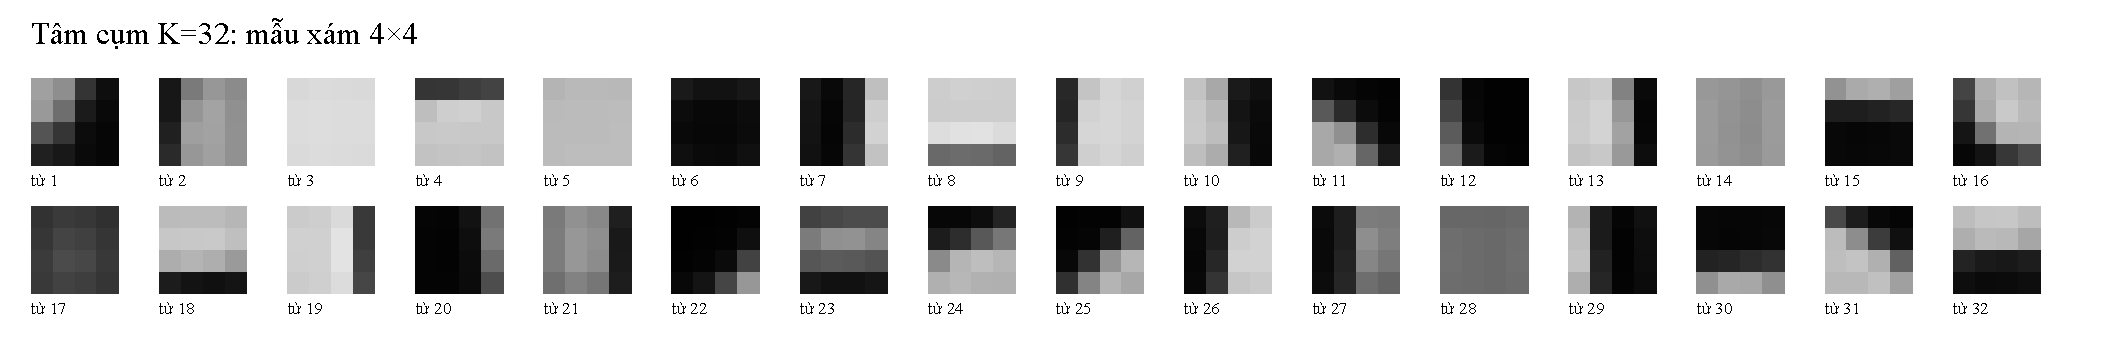
\includegraphics[width=0.88\textwidth]{codebook_centroids.pdf}
    \caption{Các descriptor tâm cụm của codebook $K=32$ ở seed 123. Mỗi ô biểu diễn một mẫu mức xám $4\times4$; số thứ tự là mã từ thị giác trong codebook.}
    \label{fig:tv3_k32_centroids}
\end{figure*}

\subsection{Phạm vi kết luận}

Trong phạm vi phân tích này, $K=32$ kết hợp với BoVW nhị phân được chọn làm cấu hình cơ sở vì tạo ra biểu diễn gọn hơn $K=64$ nhưng phong phú hơn $K=16$ theo số cặp phổ biến, đồng thời tránh đưa thêm giả định vị trí vào giao dịch chính. Đây là lựa chọn thực dụng cho mục tiêu khai phá và rà soát mẫu, không phải nghiệm tối ưu đã được chứng minh theo mọi tiêu chí. Nếu chỉ tối thiểu hóa độ méo thì các giá trị $K$ lớn hơn có lợi thế; nếu ưu tiên lượng mẫu để khảo sát thì kết quả phụ thuộc ngưỡng và tiêu chí diễn giải.

Kết quả này không đủ để kết luận BoVW nhị phân tốt hơn các biểu diễn không gian. Vì vậy, $K=32$ kết hợp BoVW nhị phân chỉ được dùng làm cấu hình cơ sở cho phần phân tích mẫu. Ngoài ra, codebook và giao dịch được tạo từ cả 70.000 ảnh, gồm cả tập kiểm thử gốc, nên các kết quả này phục vụ phân tích khai phá mẫu chứ không phải đánh giá dự đoán độc lập.

\end{document}
